\chapter{Link Budget and Final Results} \label{ch:Link}

\section{Link Budget Analysis}

To validate the feasibility of the high-rate X-band downlink, a comprehensive link budget analysis was conducted. The theoretical framework and parameter estimation for this budget rely on orbital data extracted from Systems Tool Kit (STK) combined with standard AMSAT/IARU link calculation models. While certain secondary parameters with negligible impact on the final path loss were omitted to streamline the analysis, the resulting budget is robust and accurately reflects the physical constraints of the mission.

\begin{table}[htbp]
    \centering
    \caption{Payload Downlink budget for the \textsf{CHESS} mission.}
    \label{tab:xband_downlink_budget}
    \begin{tabular}{llcccc}
        \toprule
        \textbf{Item} & \textbf{Symbol} & \textbf{Adverse} & \textbf{Nominal} & \textbf{Favourable} & \textbf{Dimension} \\
        \midrule
        Frequency & $f$ & 10.475 & 10.475 & 10.475 & GHz \\
        Data Rate & $R$ & 10 & 25 & 25 & Mbps \\
        S/C Output Power & $P$ & 0.47 & 1.48 & 5.29 & W \\
        S/C antenna Gain & $G_t$ & 17 & 19 & 21 & dBi \\
        S/C antenna HPBW & $\theta_t$ & 20.2 & 17 & 15.3 & deg \\
        S/C pointing error & -- & $\pm 7.5$ & $\pm 5$ & $\pm 3$ & deg \\
        S/C pointing loss & $L_t$ & -1.7 & -1.04 & -0.46 & dB \\
        Line loss & $L_{\theta,t}$ & -0.6 & -0.5 & -0.4 & dB \\
        EIRP & -- & 9.27 & 17 & 25.2 & dBW \\
        S/C max. altitude & $H$ & 505 & 500 & 495 & km \\
        Atmospheric Loss & $L_a$ & -1.9 & -2.1 & -2.2 & dB \\
        GS min. elevation & $\varepsilon$ & 15 & 15 & 15 & deg \\
        GS antenna Gain & $G_r$ & 40 & 40.7 & 43.1 & dBi \\
        Polarization loss & $L_{pol}$ & -0.5 & -0.3 & -0.1 & dB \\
        GS antenna HPBW & $\theta_r$ & 2.8 & 1.4 & 0.8 & deg \\
        GS Pointing error & -- & $\pm 1$ & $\pm 0.5$ & $\pm 0.25$ & deg \\
        GS pointing loss & $L_{\theta,r}$ & -1.53 & -1.53 & -1.17 & dB \\
        GS noise T$^\circ$ & $T_0$ & 148.5 & 135 & 121.5 & K \\
        GS FoM & $G_r/T$ & 15.2 & 15.7 & 16.1 & dB/K \\
        Implementation losses & $L_i$ & -2 & -2 & -2 & dB \\
        $E_b/N_0$ & -- & 4.1 & 7.1 & 18.6 & dB \\
        Required $E_b/N_0$ & -- & 2.3 & 2.3 & 2.3 & dB \\
        \midrule
        \textbf{Margin} & -- & \textbf{1.8} & \textbf{4.8} & \textbf{16.3} & \textbf{dB} \\
        \bottomrule
    \end{tabular}
\end{table}

The calculation evaluates three distinct operational scenarios: Favourable, Nominal, and Adverse. As detailed in \Cref{tab:xband_downlink_budget}, the nominal scenario yields a link margin of $4.8$ dB. According to the European Cooperation for Space Standardization (ECSS) guidelines and classical satellite communication literature \autocite{Maral2009}, a minimum margin of $3$ dB is highly recommended for nominal LEO downlinks to absorb unmodeled atmospheric attenuation or transient pointing errors. Therefore, our nominal configuration safely complies with aerospace standards. In the worst-case (Adverse) scenario, the margin is reduced to $1.8$ dB. This extremely tight tolerance highlights that employing the concatenated Convolutional and Reed-Solomon coding scheme (\Cref{sec:tm_sync_coding}) is not merely an option, but a strict requirement to maximize coding gain and successfully close the link under degraded conditions.

Furthermore, the budget deliberately assumes a conservative $2$ dB implementation loss ($L_i$). However, empirical evaluation of our Software-Defined Radio architecture demonstrates that the actual penalty is slightly lower. As illustrated by the performance evaluation in \Cref{fig:final_pipeline_performance}, the discrepancy between the theoretical standard curve and our practical software implementation is approximately $1.4$ dB. This confirms that the software receiver performs well within the established budget boundaries.

\section{Final Results and Real-Time Execution}

A central objective of this project was to verify whether standard C++ based DSP blocks in GNU Radio could sustain the mission's high-throughput requirements without relying on dedicated hardware acceleration, such as FPGAs. The transition from application-specific integrated circuits to algorithms running on Commercial Off-The-Shelf (COTS) servers introduces heavy computational constraints.

To test the system's operational limits, the complete receiver pipeline was deployed on a compact base station server (\href{https://www.galaxus.ch/fr/s1/product/geekom-a8-max-1000-go-32-go-radeon-780m-pc-58778517}{Geekom A8 Max}, featuring an AMD Radeon 780M architecture and 32 GB of RAM). Under these real-world execution conditions, the software receiver successfully sustained a stable, real-time decoding throughput of $28$ Mbps without encountering buffer overflows or frame drops. This result comfortably exceeds the nominal target of $25$ Mbps specified in \Cref{tab:xband_downlink_budget}, conclusively demonstrating that a purely software-defined architecture is fully viable for this \textsf{CHESS} mission scenario.

\begin{figure}[!ht]
    \centering
    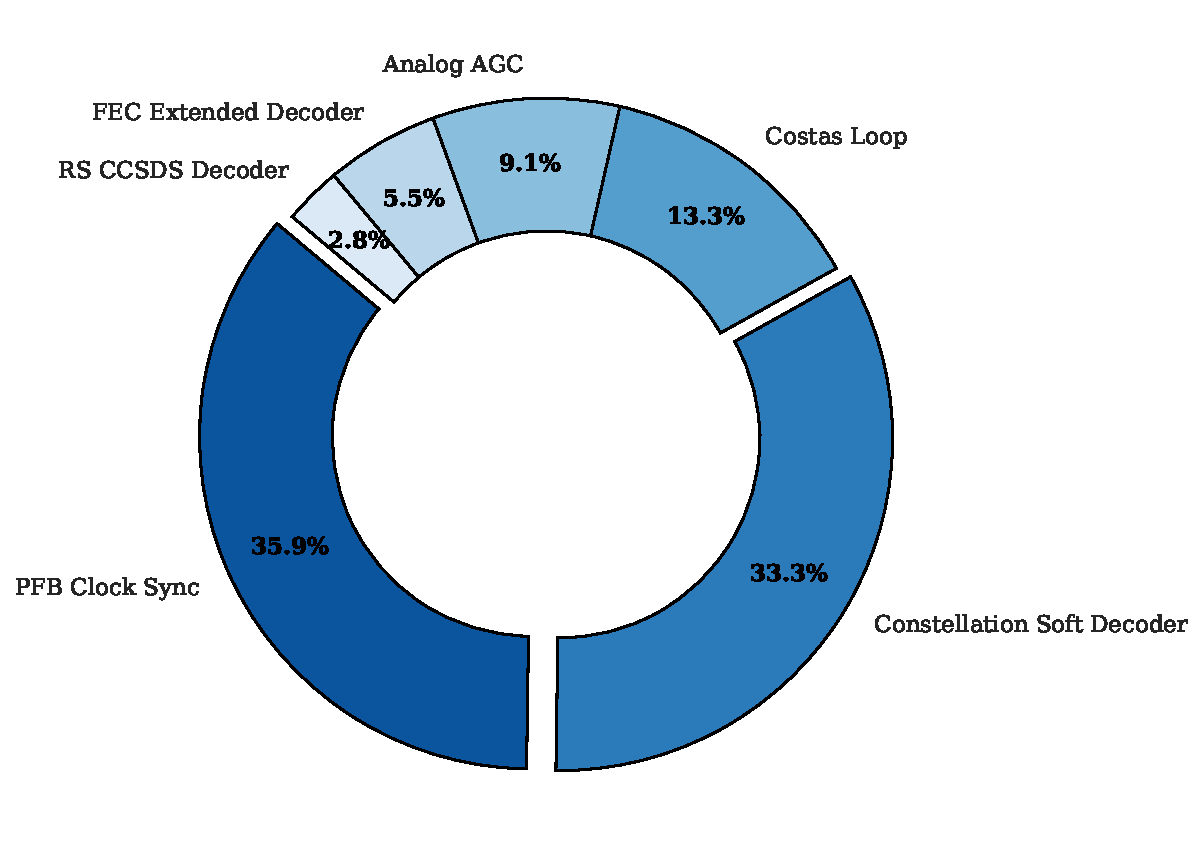
\includegraphics[width=0.6\textwidth]{figures/Inkscape/cpu_load_donut.pdf}
    \caption{Relative CPU resource allocation among the primary DSP modules of the receiver pipeline.}
    \label{fig:cpu_load}
\end{figure}

To further understand the computational bottlenecks of the system, a performance profiling analysis was conducted during the real-time execution. \Cref{fig:cpu_load} illustrates the relative CPU consumption of the most intensive signal processing blocks within the flowgraph. The remaining modules possess a negligible computational footprint. As depicted, the tracking and decoding stages --- specifically the Costas Loop, the Polyphase Clock Sync, and the Constellation Soft Decoder --- monopolize the vast majority of the system's resources. This performance distribution clearly demonstrates that if future mission profiles demand an increase in the data rate beyond $28$ Mbps, optimization efforts (such as SIMD vectorization or multi-threading) must be strictly targeted at these specific synchronization blocks.

\begin{figure}[htbp]
    \centering
    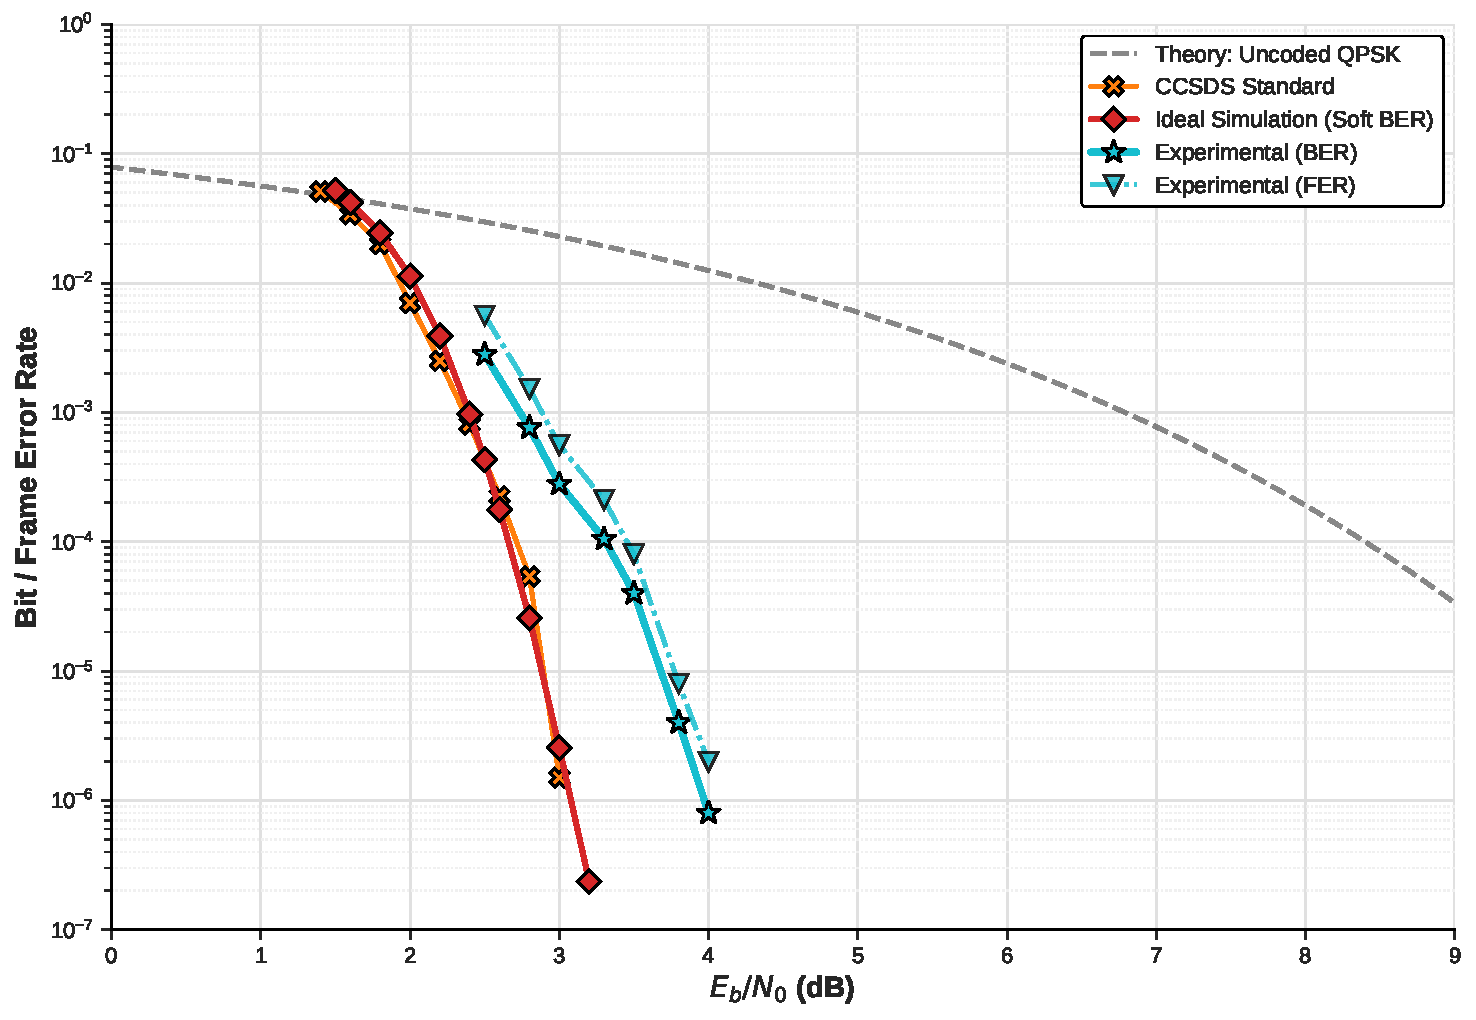
\includegraphics[width=1\linewidth]{figures/Inkscape/Final_Performance_Plot.pdf}
    \caption{Final bit and frame error rate performance of the complete SDR pipeline. The experimental curve illustrates the real-time execution including Doppler tracking and dual-branch synchronization, compared against the ideal simulated soft-decoding performance, the theoretical CCSDS limit, and the uncoded QPSK baseline.}
    \label{fig:final_pipeline_performance}
\end{figure}